\chapter[Estudo Exploratório]{Estudo Exploratório}

Para a realização da proposta foi adotada a atividade de exploração, devido ao grau de intervenção foi baixo. O paradigma empregado foi experimental e a análise realizada foi semi-quantitativa, pois associou-se observação a medição de alguma tendência. Os passos adotados foram, em sua maioria, os sugeridos por \citeonline{travassos2011experimentaccao}. O estudo exploratório foi concebido com base nos objetivos levantados na proposta de estudo \ref{propostaestudo}, e em cada foi conduzido. Na Seção \ref{sec:planejamento} consta a descrição de como o estudo foi preparado. As etapas de execução estão na Seção \ref{sec:execucao}, seguido pelos resultados presentes na Seção \ref{sec:resultados} e por fim, a análise e discussão está na Seção \ref{sec:discussao}.

\section{Planejamento \label{sec:planejamento}}

Para conseguir a realização do estudo exploratório foi necessário planejar três principais aspectos: a geração de dados de teste, a execução da cobertura de código e o parâmetro de estudo, ou seja, o código no qual as etapas anteriores utilizaria.

A princípio, buscou-se trabalhar com o menor escopo possível, escolhendo um algoritmo genético simples que se assemelha a definição formal. E a partir disso definir uma função objetivo para a geração de dados de teste. O algoritmo adotado foi o presente no livro de \cite{russell2016artificial}, e o parâmetro de estudo escolhido foi o \textit{Scikit-learn} \cite{pedregosa2011scikit}. Nas primeiras manipulações, foi constatado que seria um trabalho fastidioso e que não estaria de acordo com a proposta de estudo. Por isso, contornou-se o planejamento para a escolha de uma ferramenta de geração de dados de teste que está em um estado mais avançado. 

A seleção aconteceu ao se consultar a competição de ferramentas para testes unitários em Java, que teve sua quinta edição em 2017 e faz parte do congresso de SBST \cite{panichella2017java}. Foi escolhido então, a ferramenta EVOSUITE\footnotemark \footnotetext{\url{http://www.evosuite.org/}}, ganhadora da última edição, que gera automaticamente casos de teste com asserções para classes escritas em código Java \cite{fraser2011evosuite}. 

A EVOSUITE aplica uma abordagem multiobjetivo para os critérios de busca, ou seja, constrói a função objetivo da otimização baseando em mais do que no critério de cobertura de código. Adicionalmente, ela possui uma série de parâmetros para a execução, como a seleção de qual algoritmo utilizar, visto que tem suporte mais de um, o tempo de busca para otimização, a quantidade máxima de iterações, o tamanho da população, no caso dos algoritmos genéticos, entre outros. 

Como parâmetro de estudo foi escolhido o projeto Jsoup\footnotemark \footnotetext{\url{https://jsoup.org/}}, que é uma biblioteca Java para trabalhar com HTML, que fornece uma API para extrair e manipular dados de páginas web. É um projeto de código livre fácil de manipular e compreender \cite{hedley2009jsoup}. Além disso, ela maior se adequa a EVOSUITE por ser orientada a objeto e por estar em Java. Uma opção melhor, mas que prejudicaria bastante os testes por causa do tempo de teste é o conjunto de projetos denominado de SF100 \cite{TOSEM_evaluation}, criado especialmente para teste de integração das novas versões do EVOSUITE.

Com a definição da ferramenta e do projeto, partiu-se então para o planejamento da execução dos experimentos de exploração. De acordo com o propósito, viu-se a necessidade de ter várias massas de dados que se distinguem no tempo. Assim, sendo a geração de dados de teste e a execução dos mesmos serão realizados a cada período de tempo acrescido. A estratégia será adotada justamente para se conseguir observar o comportamento de tais atividades.

\section{Execução \label{sec:execucao}}

A execução do estudo exploratório fez uso adicional das seguintes ferramentas:

\begin{enumerate}
    \item OpenClover\footnotemark \footnotetext{\url{http://openclover.org/}}: ferramenta de cobertura de código para Java, Groovy e AspectJ.
    \item Matplotlib\footnotemark \footnotetext{\url{https://matplotlib.org/}}: biblioteca de plotagem de gráficos 2D em Python.
    \item Pandas\footnotemark \footnotetext{\url{https://pandas.pydata.org/}}: biblioteca que fornece estruturas de dados de alto desempenho e ferramentas de análise de dados para a linguagem de programação Python.
\end{enumerate}

O OpenClover foi selecionado devido a sua facilidade de customização da execução e de extração dos dados de cobertura de código. A adoção do Matplotlib junto com o Pandas se deve a simplicidade de construção do tipo de gráfico escolhido. Todas as ferramentas utilizadas são gratuitas e de código aberto.

O passo a passo da execução dos experimentos podem ser vistos abaixo. Foram criados scripts (\ref{scripts}) que sistematizaram e garantiram a replicabilidade dos procedimentos. Eles foram executados em um ambiente computacional com o processador Intel Core i7-7700 CPU @3.60GHz e com 16GB de memória RAM.

\subsection{Execução dos ensaios de teste}

Etapa em que o script run.sh (\ref{run.sh}) é executado. A sua aplicação é realizada na pasta anterior ao do projeto em que vai se executar a ferramenta EVOSUITE, da seguinte maneira: \mintinline{shell}{./run.sh TARGET_CLASS PATH_PROJECT SUBPATH_PROJECT}. É necessário a passagem de três parâmetros, o \mintinline{shell}{TARGET_CLASS} que é o nome da classe incluindo o pacote que vai ser executado, o \mintinline{shell}{PATH_PROJECT} que se refere a pasta do projeto que vai ser testado e o \mintinline{shell}{SUBPATH_PROJECT} que é a estrutura de diretório que o projeto se encontra. 

Um exemplo do script para a classe \textit{Parser} do pacote \textit{parser} que é testada e a cobertura de código verificada executado é o seguinte: 

\mintinline{shell}{./run.sh org.jsoup.parser.Parser jsoup org/jsoup/parser}

Em cada ensaio, são executadas 10 massas de dado que variam de 2 em 2 segundos até o limite de 20 segundos. O \mintinline{shell}{-Dsearch_budget} é a propriedade de execução do EVOSUITE que delimita o tempo de busca. O algoritmo fixado pelo propriedade \mintinline{shell}{-Dalgorithm} foi o \mintinline{shell}{STANDARD_GA}. Com a geração dos testes pela ferramenta, é executada a cobertura com o OpenClover que vai guardando o histórico em um diretório diferente do projeto. O EVOSUITE, por sua vez, cria o diretório \textit{evosuite-report} e armazena as estatísticas no arquivo \textit{statistics.csv}.

\subsection{Extração das métricas da execução da cobertura de código}

Essa etapa é responsável for extrair as métricas de tempo e cobertura de código a partir dos relatórios salvos pelo OpenClover durante a etapa anterior. Para isso, foi criado o script \mintinline{shell}{./extract.sh} (\ref{extract.sh}), que é executado no diretório \textit{clover-history} e produz o arquivo \textit{statistics-execution.csv}. 

Um detalhe dessa etapa é que a cobertura pela ferramenta se dá pela divisão dos elementos cobertos pelo total de elementos. O elemento no caso são os critérios de cobertura da OpenClover, que vão além de a quantidade de linhas do programa.

\subsection{Manipulação dos dados}

Essa etapa é bem simples, consiste apenas na extração manual do dados específicos da classe que se deseja do arquivo \textit{statistics.csv} produzido pelo EVOSUITE. Isso porque, ele guarda o histórico de todas as execuções. Um passo importante também e retirar o aquivo anteriormente produzido (\textit{statistics-execution.csv}) para o diretório aonde os gráficos serão gerados.

\subsection{Geração dos gráficos} 

Para a geração dos gráficos foi produzido o script em Python \textit{plot.py} (\ref{plot.py}). Sua execução necessita do nome do arquivo, que por padrão adotou-se o nome da classe e o tipo, sendo geração ou execução (\mintinline{python}{python plot.py FILENAME TYPE}). Abaixo segue o exemplo para a classe \textit{Parser}:

\mintinline{python}{python plot.py jsoup.parser.parser generation} 
 
\mintinline{python}{python plot.py jsoup.parser.parser execution}

\section{Resultados \label{sec:resultados}}

A princípio, não obedecendo os passos anteriormente citados, foi realizado um ensaio com todas as classes do pacote \textit{parser} definindo 30 massas de dados com 1 segundo de intervalo para cado uma. Para cada massa de dado foi feita a média da cobertura e dp tempo para geração das 14 classes presentes no pacote. A Figura \ref{fig:genJsoup} representa na linha contínua de azul, a porcentagem cobertura de código, e na linha tracejada laranjada, o esforço computacional de tempo expresso em milissegundos. Tal simbolização foi seguida pra os outros gráficos apresentados.

\begin{figure}[H]
	\centering
	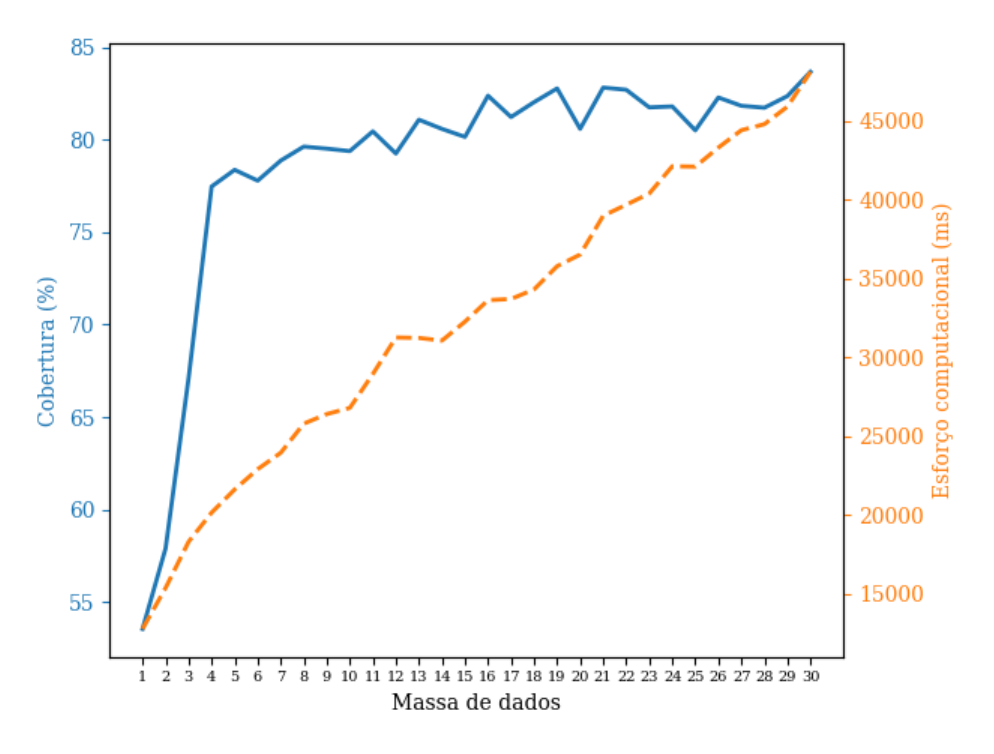
\includegraphics[scale=0.6]{figuras/jsoup.parser_generation.eps}
	\caption{Geração de dados de teste para o pacote \textit{jsoup.parser}}
	\label{fig:genJsoup}
\end{figure}

Após isso, foram executados os procedimentos para as classes do pacote \textit{parser}. Para a apresentação dos resultados, bem como para a discussão, foram escolhidos três classes: a \textit{Parser}, a \textit{Tag} e a \textit{HtmlTreeBuilder}. A \textit{Parser}, com os resultados expressos na Figura \ref{fig:JsoupParser}, tem a sua importância por analisar um HTML e converter em um \textit{Document} (classe interna de representação do DOM). Além disso, é uma classe que possui várias estruturas de dados importantes do projeto. 

\begin{figure}[H]
\centering
\begin{subfigure}{.5\textwidth}
    \centering
    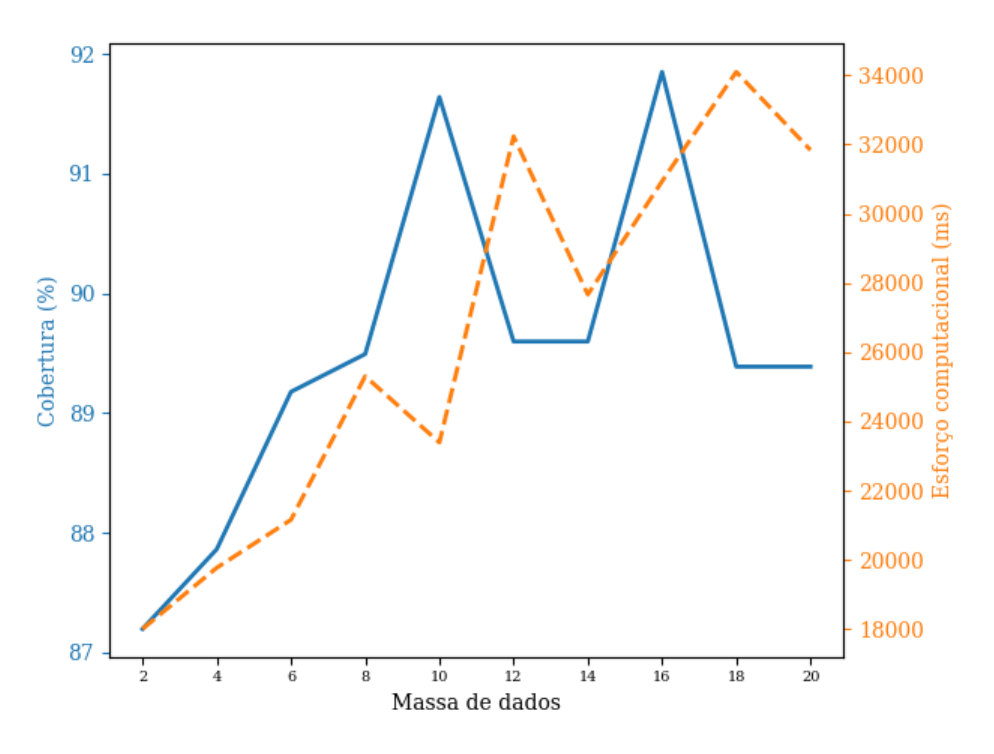
\includegraphics[scale=0.5]{figuras/jsoup.parser.parser_generation.eps}
    \caption{Geração dos testes}
    \label{fig:genJsoupParser}
\end{subfigure}%
\begin{subfigure}{.5\textwidth}
    \centering
    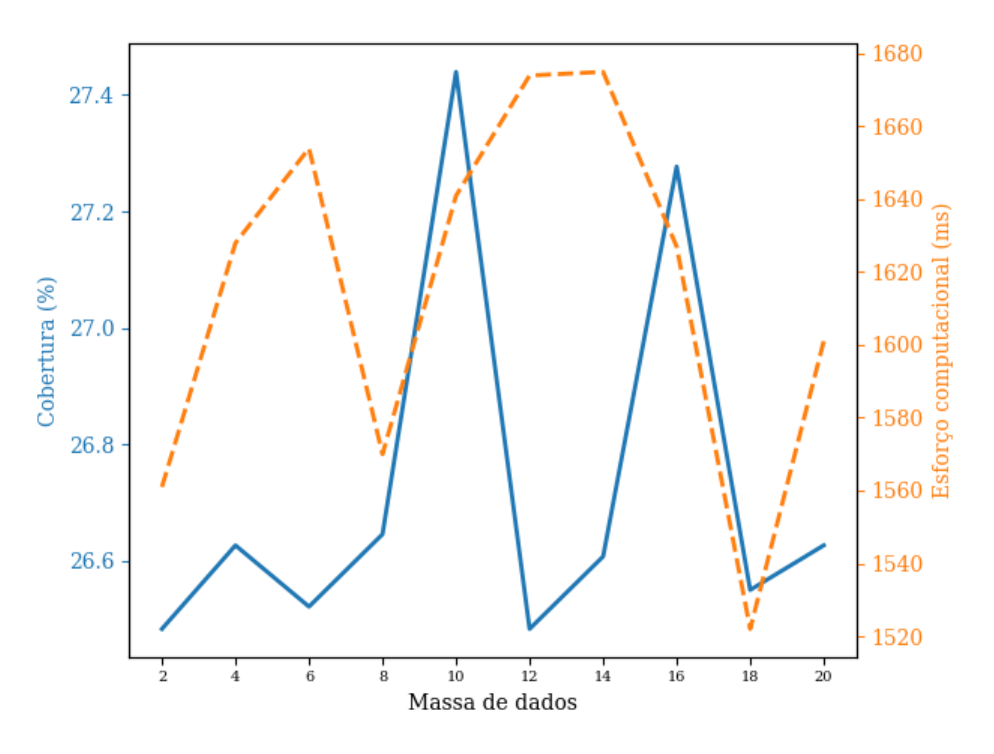
\includegraphics[scale=0.5]{figuras/jsoup.parser.parser_execution.eps}
    \caption{Execução dos testes}
    \label{fig:execJsoupParser}
\end{subfigure}
\caption{Classe \textit{jsoup.parser.Parser}}
\label{fig:JsoupParser}
\end{figure}

Para testar uma classe mais simples, foi escolhido a classe \textit{Tag}, que é uma classe de definição e que serve de representação para uma tag em HTML. A Figura \ref{fig:JsoupTag} consolida a execução dos passos para a classe.

\begin{figure}[H]
    \centering
    \begin{subfigure}{.5\textwidth}
        \centering
        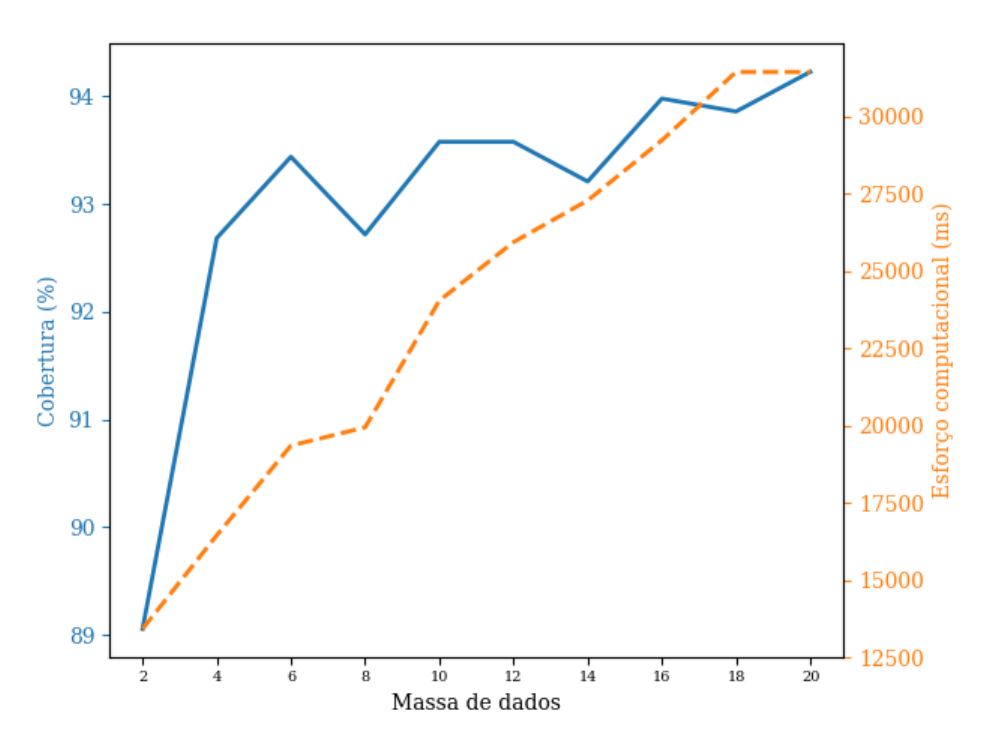
\includegraphics[scale=0.5]{figuras/jsoup.parser.tag_generation.eps}
        \caption{Geração dos testes}
        \label{fig:genJsoupTag}
    \end{subfigure}%
    \begin{subfigure}{.5\textwidth}
        \centering
        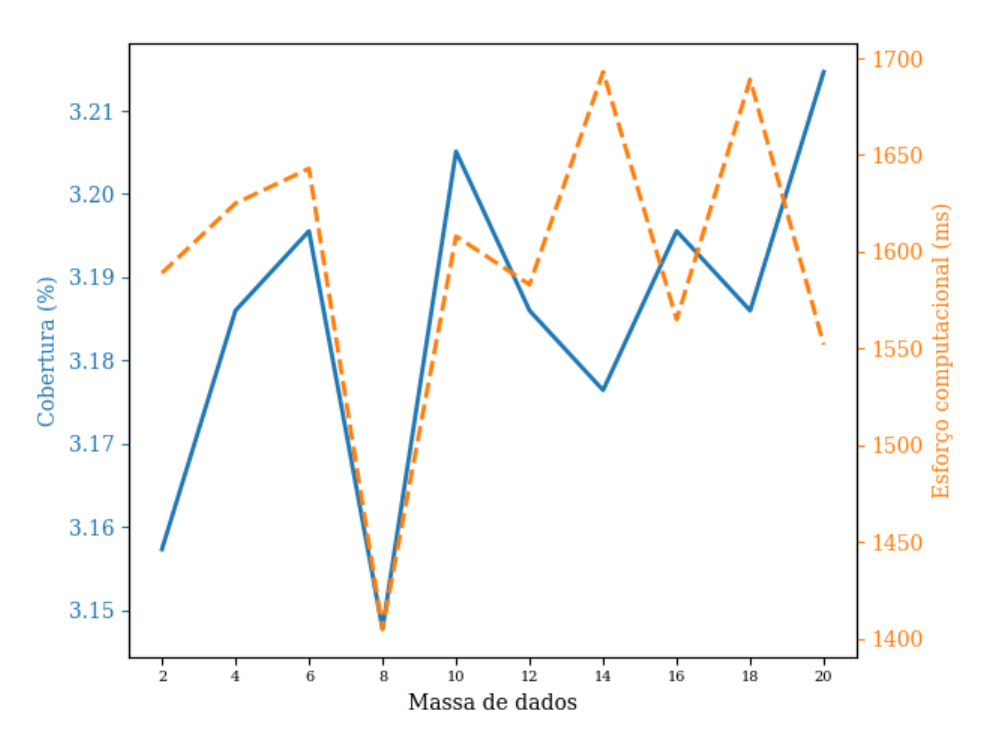
\includegraphics[scale=0.5]{figuras/jsoup.parser.tag_execution.eps}
        \caption{Execução dos testes}
        \label{fig:execJsoupTag}
    \end{subfigure}
    \caption{Classe \textit{jsoup.parser.Tag}}
\label{fig:JsoupTag}
\end{figure}

% \begin{figure}[H]
% 	\centering
% 	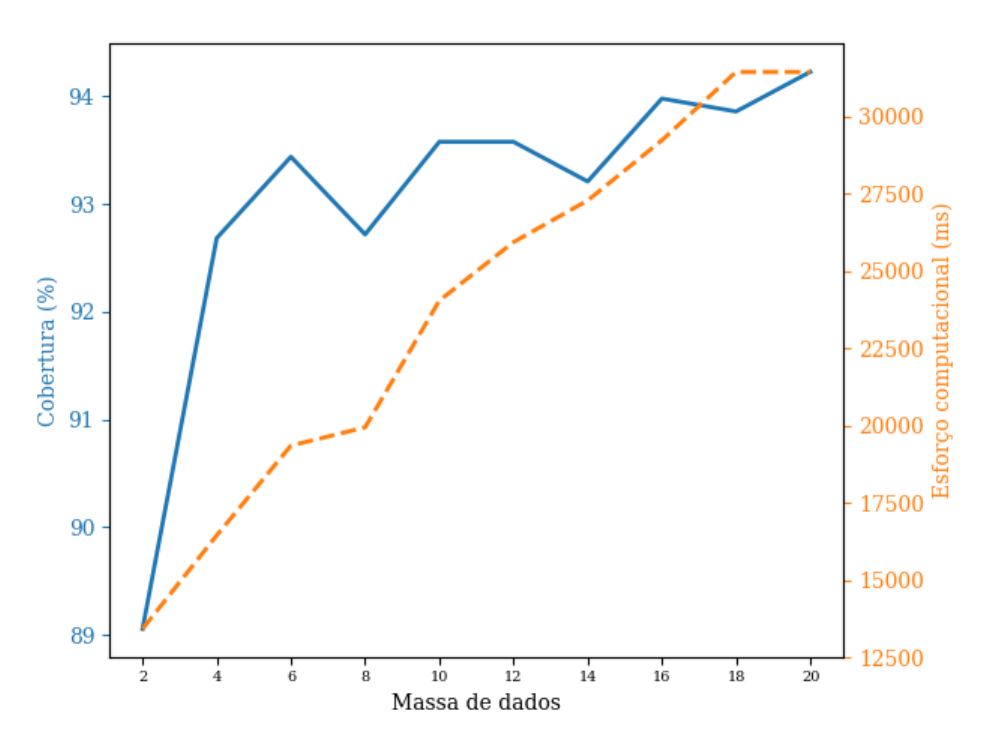
\includegraphics[scale=0.6]{figuras/jsoup.parser.tag_generation.eps}
% 	\caption{Geração de dados de teste para a classe \textit{jsoup.parser.Tag}}
% 	\label{fig:genJsoupTag}
% \end{figure}

% \begin{figure}[H]
% 	\centering
% 	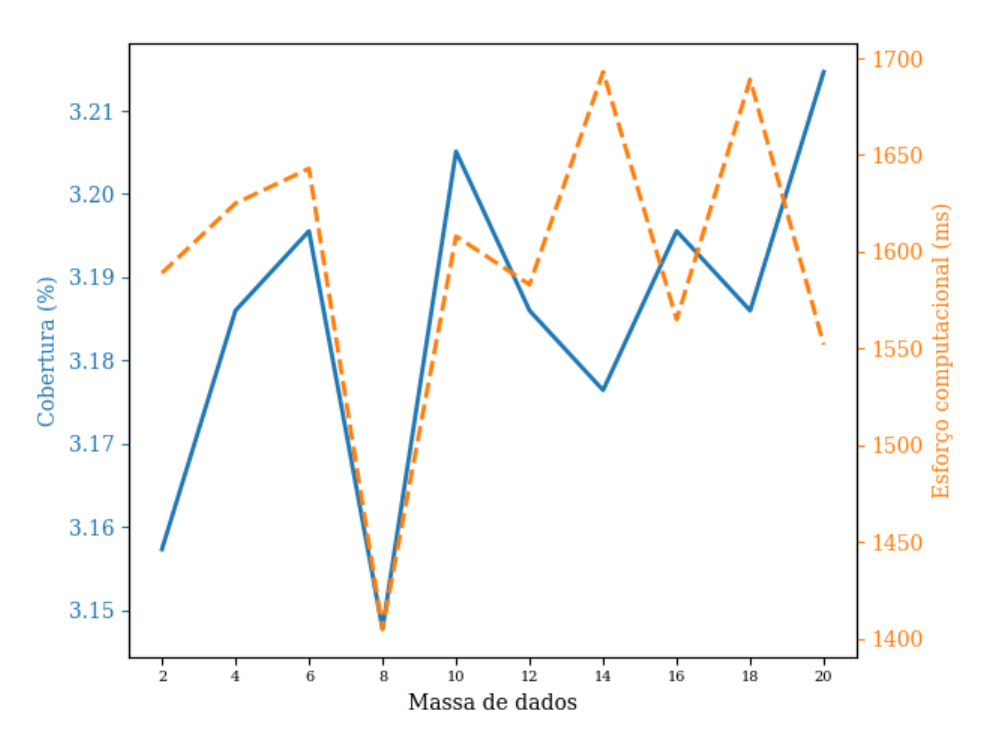
\includegraphics[scale=0.6]{figuras/jsoup.parser.tag_execution.eps}
% 	\caption{Execução dos teste da classe \textit{jsoup.parser.Tag}}
% 	\label{fig:execJsoupTag}
% \end{figure}

Por fim, buscou-se escolher uma classe bem robusta e essencial a finalidade do pacote. Por isso, a classe \textit{HtmlTreeBuilder} foi selecionada. Ela é responsável pela criação da estrutura de árvore de uma página HTML, estruturando todo o DOM. Os resultados para a classe podem ser encontradas na Figura \ref{fig:JsoupHtmlTreeBuilder}.

\begin{figure}[H]
    \centering
    \begin{subfigure}{.5\textwidth}
        \centering
        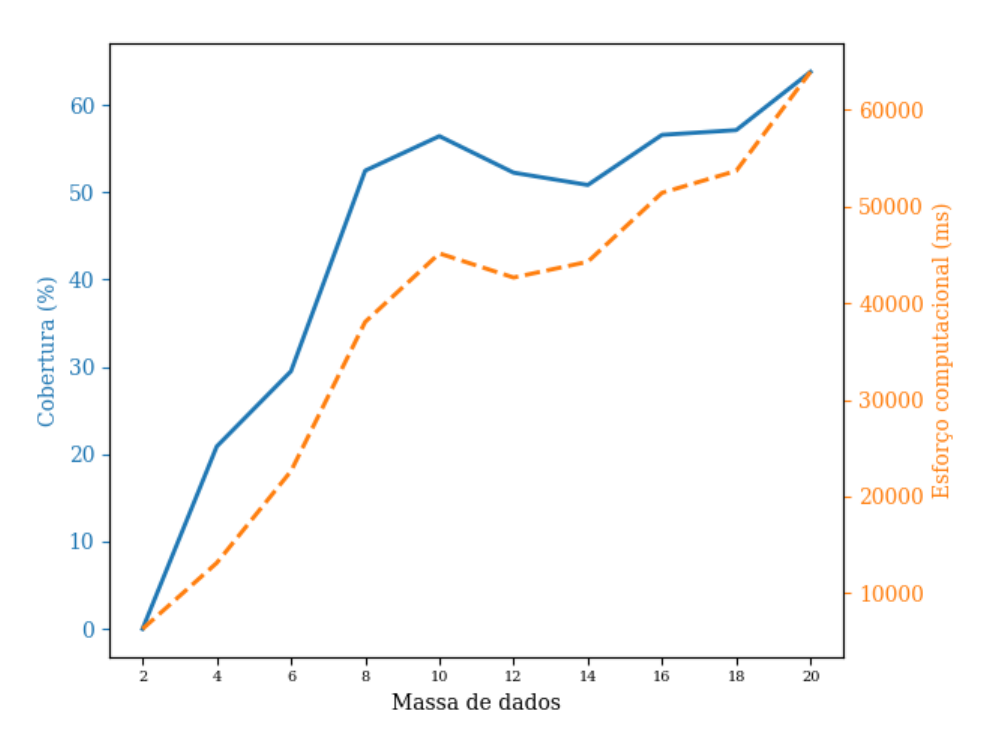
\includegraphics[scale=0.5]{figuras/jsoup.parser.htmltreebuilder_generation.eps}
        \caption{Geração dos testes}
        \label{fig:genJsoupHtmlTreeBuilder}
    \end{subfigure}%
    \begin{subfigure}{.5\textwidth}
        \centering
        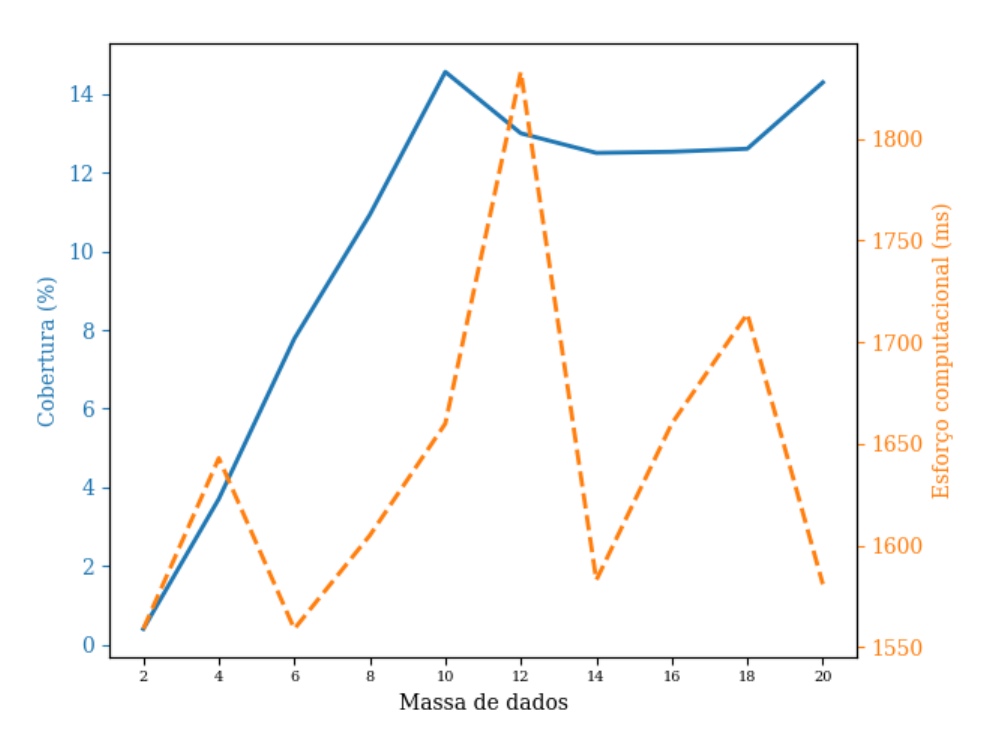
\includegraphics[scale=0.5]{figuras/jsoup.parser.htmltreebuilder_execution.eps}
        \caption{Execução dos testes}
        \label{fig:execJsoupHtmlTreeBuilder}
    \end{subfigure}
    \caption{Classe \textit{jsoup.parser.HtmlTreeBuilder}}
\label{fig:JsoupHtmlTreeBuilder}
\end{figure}

\section{Discussão \label{sec:discussao}}

A partir dos resultados apresentados foram levantados vários pontos para se discutir. Dividiu-se a discussão em três momentos: a geração dos testes, a execução dos testes e a relação entre ambos momentos. Para os dois primeiros, tanto a porcentagem de cobertura como o tempo em milissegundos foram analisados. 

Um detalhe que é importante ressaltar é que as escalas dos gráficos não estão consistentes. Optou-se pela ampliação da função do que o congelamento de uma escala no eixo da abscissa e nos das ordenadas. Alguns gráficos, por exemplo, tem a cobertura variando na segunda casa decimal. Por outro, lado outros crescem em inteiros. A escolha por não fixar foi motivada para conseguir melhor observer o comportamento.

\subsection{Geração dos Testes}

De maneira geral, é possível observar que a cobertura de testes têm um comportamento logarítmico ao se analisar o comportamento gráfico. Logo nas primeiras massas de dados, em uma média até 6, a cobertura de código já conseguem valores altos e consistentes. Após isso, em geral começa a crescer de uma maneira mais lenta, tendo em alguns momentos declives e depois picos. 

O fenômeno relatado pode ser explicado pela variabilidade que se deu na geração dentro do algoritmo genético. Seus indivíduos sofreram recombinação e isso levou a uma geração menos adaptava do que a anterior, processo natural do algoritmo genético. De qualquer forma, não é toda a população que regride, o que faz com que continuando as gerações e as seleções a adaptação a função objetivo tenda a crescer. 

A Figura \ref{fig:JsoupParser} representa muito bem isso, que durante a massa de dados 8 até a 20 o que se tem são dois picos e duas depressões. O segundo pico e a segunda depressão são mais agudas, o que leva a entendem que a busca está conseguindo adentrar mais profundamente, mas que isso está gerando uma inconstância na cobertura. Em todas as figuras é possível notar em algum momento esse comportamento de oscilação.

Diferente da cobertura de código, o tempo de execução na geração de testes aparenta ter uma relação mais direta com a massa de dados. Na maioria dos casos a função gráfica tende a ter o comportamento linear. Por exemplo, na Figura \ref{fig:JsoupTag} o tempo de execução cresce a medida que as massas de dados vão crescendo também.

Entretanto, algumas oscilações são visíveis. Na Figura \ref{fig:JsoupParser} é possível observar que nos momentos de depressão da cobertura de código mais se elevou o esforço computacional. Essa é uma alteração brusca do comportamento, pois geralmente o que se nota são pequenas diferenças.

Em alguns momentos faz-se a análise que ambas variáveis não tem uma relação explícita. Uma figura que demostra de uma maneira bem particular que existe uma dependência entre cobertura de código e esforço computacional é a Figura \ref{fig:JsoupHtmlTreeBuilder}. Nela, verifica-se que a medida cobertura vai crescendo e sofrendo suas oscilações o tempo em milissegundos vai seguindo só que em escala menor.

\subsection{Execução dos Testes}

A cobertura na execução dos testes teve, em suma maioria, variações constantes, mas em uma escala bem reduzida, como é visto na Figura \ref{fig:JsoupTag}. No qual a maior diferença é de apenas 0.05\% de cobertura de código. 

Como a cobertura na execução foi analisada como um todo, é interessante ver o impacto da classe \textit{Parser}, que representa quase que 1/3 do que seria toda a cobertura do projeto. Enquanto que a classe \textit{Tag} quase não tem valor para o todo, ficando abaixo dos 4\%.

O tempo na execução por sua vez, impressiona que em nenhum dos casos passou de 2 segundos, valor baixo ao se comparar, por exemplo, com os 60 segundos que se adquiriu na geração de testes da classe \textit{HtmlTreeBuilder}. Todavia, para a evolução das massas de dados não é possível verificar muita correspondência no tempo, já que em todos os casos existem oscilações.

Em alguns momentos é possível verificar uma relação direta entre a cobertura e em outros não. De modo que, na Figura \ref{fig:JsoupParser} nota-se que na massa de dados 8 quando a cobertura decresce, o tempo também diminui. Mas que por outro lado, na massa de dados 14 e na massa de dados 18, em que também a cobertura de código caiu, o tempo de execução aumentou. Logo não é possível estabelecer uma relação direta, mas observa-se que existe um certo grau de influência.

\subsection{Relação entre a Geração e a Execução dos Testes}

Observando tanto cobertura de código quanto o esforço computacional, nota-se uma maior relação da cobertura de código entre a geração e a execução dos testes. O tempo, por sua vez, vínculo com a cobertura em cada momento, mas entre as etapas não é possível ter uma boa inferência.

A vinculação entre a cobertura de código é bem expressada na Figura \ref{fig:JsoupHtmlTreeBuilder}, que de uma maneira mais contínua, a execução é impactada pela geração. Tanto que nas massas de dados em que se tem um declínio da cobertura, o gráfico de execução também é enternecido. Com o crescimento da cobertura na geração de dados de teste, a cobertura da execução também volta a crescer. 

Nota-se que o ponto de equilíbrio entre tal relação está ligado com as oscilações que começa a sofrer. E neste momento que está se buscando mais, mas que as mesmo tempo tem-se pouca evolução. Interromper a geração em um ponto de pico dessas oscilações pode ser um bom parâmetro para a função objetivo e tende a diminuir o esforço computacional.

\subsection{Ameaças a Validade}

As variáveis de interesse, cobertura de código e esforço computacional expresso no tempo de execução apresentam algumas ameaças de validade, quem tem a sua origem na natureza e na especificidade de cada ferramenta. O projeto também escolhido, assim como as classes também são ameaças ao estudo. Entretanto, ambos já foram discutidos anteriormente, por isso, a seguir segue a discussão sobre a cobertura de código e o tempo de execução.

\subsubsection{Cobertura de Código}

A cobertura de código programada na EVOSUITE é diferente na OpenClover. A ferramenta de geração trabalha com a cobertura da classe com o qual está se produzindo os testes, por isso, a sua porcentagem sempre é superior a da ferramenta de execução dos testes. Isso, porque a OpenClover considera todos os elementos presentes no software.

Mesmo o apresentado sendo uma ameaça é interessante considerar todos os elementos ao se calcular a cobertura de código, pois é possível ver o impacto da classe sobre o todo. Assim como a visão dada pela EVOSUITE mostra o comportamento da cobertura local de uma classe. Outro fator é que não se tem a certeza de que a implementação para o cálculo de cobertura levam em conta os mesmos fatores. 

\subsubsection{Tempo de Execução}

O tempo de execução também é divergente entre a ferramenta de geração e a de execução. A OpenClover tem seu tempo de execução muito variado porque tem passos que dependem muito da instrumentação do código para a realização do teste. Além, do fato que ao ocorrer exceções ou desvios durante a execução podem haver acréscimos ou descontos do tempo total estimado. 

A EVOSUITE também produz um tempo variável, pois somente encerra quando a o processo de otimização da geração que está sendo evoluída finaliza. Assim como na anterior, quebras ou geração de descendentes no algoritmo genético vão gerar tempo adicional além do que a massa de dados estipulou.

